\documentclass[9pt]{beamer}


\mode<presentation>
{
\usetheme{Singapore} %use default if problems or  Singapore or 
  % or ... https://deic-web.uab.cat/~iblanes/beamer_gallery/index_by_theme.html
\usefonttheme{serif}  
}
\setbeamertemplate{footline}[frame number]
\usepackage{booktabs}
\usepackage{color}

\usepackage[english]{babel}
% or whatever

\usepackage[latin1]{inputenc}
% or whatever

\usepackage{times}
\usepackage[T1]{fontenc}
% Or whatever. Note that the encoding and the font should match. If T1
% does not look nice, try deleting the line with the fontenc.
\usepackage[super]{nth}
\usepackage{xcolor}
\usepackage{relsize} %large math 

\usepackage{graphicx} % to insert the logo

\usepackage{hyperref}
\hypersetup{
  colorlinks   = true, %Colours links instead of ugly boxes
  urlcolor     = blue, %Colour for external hyperlinks
  linkcolor    = blue, %Colour of internal links
  citecolor   = red %Colour of citations
}

\usepackage[font=scriptsize,skip=1pt]{caption}

\setbeamertemplate{caption}[numbered]

\title [Oligopolistic ABM] % (optional, use only with long paper titles)
{From a theoretical oligopolistic model to a generative agent-based simulation}

\author[] % (optional, use only with lots of authors)
{P.~\href{https://terna.to.it}{Terna}\inst{1~2} \and M.~Mazzoli\inst{3} \and M.~Morini\inst{4~5}  }
% - Give the names in the same order as the appear in the paper.
% - Use the \inst{?} command only if the authors have different
%   affiliation.


\institute[] % (optional, but mostly needed)
{
  \inst{1}%
 University of Torino, Italy
  \and
 \inst{2}%
  Fondazione Collegio Carlo Alberto, Honorary Fellow, Italy
 \and
  \inst{3}%
 University of Genova, Italy 
  \and
  \inst{4}%
  Credimi S.p.A., Milano, Italy
  \and
  \inst{5}%
 Ronin Institute, Montclair, New Jersey, US
  }
% - Use the \inst command only if there are several affiliations.
% - Keep it simple, no one is interested in your street address.

\date[] % (optional, should be abbreviation of conference name)
{\href{http://proteusfoundationseries.org/event/first-international-workshop-on-agentization-rendering-conventional-models-with-agent-based-computing/}{Agentization}---September 15-17, 2021}

\begin{document}


%%%%%%%%%%%%%%%%%%%%%%%%%%%%%%%%%%%%%%%%%%%%%%%%%%%%%%%%%
\begin{frame}
\noindent\makebox[\linewidth]{\rule{\paperwidth}{0.4pt}}

\titlepage

\end{frame}

%%%%%%%%%%%%%%%%%%%%%%%%%%%%%%%%%%%%%%%%%%%%%%%%%%%%%%%%%
\begin{frame}{Outline}

  \tableofcontents
  % You might wish to add the option [pausesections]
\end{frame}

%%%%%%%%%%%%%%%%%%%%%%%%%%%%%%%%%%%%%%%%%%%%%%%%%%%%%%%%%
\section{A book on \emph{Rethinking Macroeconomics with Endogenous Market Structure}}

\subsection{Starting questions}

%%%%%%%%%%%%%%%%%%%%%%%%%%%%%%%%%%%%%%%%%%%%%%%%%%%%%%%%%
\begin{frame}{Starting questions}

%\footnote{mazzoli_morini_terna_2019}

\begin{columns}[T]
\begin{column}{.6\textwidth}
\begin{block}{}
% Your text here

\begin{itemize}

\item
Do entry, exit and changes in market structure affect the macroeconomy?

\item Is there a link between the strategic interactions among oligopolistic firms and the macroeconomic equilibrium?

\end{itemize}

\smallskip
\small
This questions are certainly not trivial in modern economies, where large oligopolistic firms play a relevant role and so many meetings among statesmen have the explicit scope of promoting contracts for some large and important firms of their countries. 

However, surprisingly enough, the most popular theoretical models in the modern macroeconomic literature hardly see any explicit formalization for the macroeconomic effects of changes in market structure, entry, exit and strategic interactions among oligopolists.
     
\end{block}
\end{column}

 \begin{column}{.4\textwidth}
 \begin{block}{}
% Your image included here
 
\includegraphics[scale=0.25]{cover.png}
  \end{block}
  \end{column}
    
\end{columns}


\smallskip

\noindent\rule{8cm}{0.4pt}
\scriptsize

Mazzoli, M., Morini, M., and Terna, P. 2019. \emph{Rethinking Macroeconomics with Endogenous Market Structure}. Cambridge University Press.

\end{frame}

%%%%%%%%%%%%%%%%%%%%%%%%%%%%%%%%%%%%%%%%%%%%%%%%%%%%%%%%%
\section{Theoretical analysis}


%%%%%%%%%%%%%%%%%%%%%%%%%%%%%%%%%%%%%%%%%%%%%%%%%%%%%%%%%
\subsection{Main assumptions}

%%%%%%%%%%%%%%%%%%%%%%%%%%%%%%%%%%%%%%%%%%%%%%%%%%%%%%%%%
\begin{frame}{Interactions among oligopolistic firms}

We introduce a new macromodel where entry, exit and strategic interactions among oligopolistic firms are explicitly formalized and may generate macroeconomic fluctuations. 

About macroeconomic impact of business formation we refer to Gabaix (2011). His ``granular hypothesis'' was initially studied by Jaimovich and Rebelo (2009). 

\bigskip
\bigskip
\bigskip
\bigskip
\bigskip


\noindent\rule{8cm}{0.4pt}
\scriptsize


Gabaix, X. 2011. The granular origins of aggregate fluctuations. \emph{Econometrica}, \textbf{79}(3), 733?72.

Jaimovich, N., and Rebelo, S. 2009. Can news about the future drive the
business cycle? \emph{American Economic Review}, \textbf{99}(4), 1097--118.

\end{frame}

%%%%%%%%%%%%%%%%%%%%%%%%%%%%%%%%%%%%%%%%%%%%%%%%%%%%%%%%%
\subsection{Outputs and aggregate demand}


%%%%%%%%%%%%%%%%%%%%%%%%%%%%%%%%%%%%%%%%%%%%%%%%%%%%%%%%%
\begin{frame}{Outputs}

The output of each firm is given by the production function, where $\psi _{i,t}$ is a positive or negative shock:

\begin{equation}
\varphi _{i,t}=\Lambda L_{i,t}^{\alpha }+\psi _{i,t}
\end{equation}

Summing up, with $P_t$ the aggregate price level (as weighted average of prices, jointly determined by the strategic behavior of the oligopolistic firms) and having $\psi _{i,t}$ a zero average:

\begin{equation}
Y_{t}=P_{t}\Lambda \overset{H_{t}}{\underset{i=1}{\sum }}L_{i,t}^{\alpha}
\end{equation}

\smallskip
\small
$H_{t}$ is is the total number of oligopolistic firms operating at time t;

$\Lambda$ the usual constant parameter capturing technology shocks;

$L_{i,t}$ the total amount of labour employed at time $t$ by firm $i$;

$\psi _{i,t}$ an idiosincratic stochastic shock reflecting (i) the Cournot-Nash equilibrium among the oligopolisti firms is in mixed strategies, herefore stochastic, plus unpredictable events (e.g., conflicts with the workers).

\end{frame}

%%%%%%%%%%%%%%%%%%%%%%%%%%%%%%%%%%%%%%%%%%%%%%%%%%%%%%%%%
\begin{frame}{Aggregate demand}

The microfounded optimization problem of the heterogeneous consumers with the same preferences but different budget constraint (depending on wether they are workers, new entrants or incumbent entrepreneurs) yields the following aggregate demand:

\begin{eqnarray}
D(\cdot )_{t} &=&\frac{\Omega (R_{t})}{P_{t}}\{A_{t}+((1+r_{t})(1+\iota
)^{-1}\sum_{i=0}^{\infty }[(1+E\left( r_{t+i}\right) (1+\iota )]^{-i}\cdot 
\notag \\
&&\cdot E(n_{t+i}(W_{t+i}+h_{t+i}^{e}\Pi _{t+i}^{e}+h_{t+i}^{in}\Pi
_{t+i}^{in}))\}  \label{per capita distrib cons_1}
\end{eqnarray}

\small

$\Pi_{t+i}^{in}$ and $\Pi _{t+i}^{e}$ are the nominal profits of the incumbent and new entrants entrepreneurs;

$r_{t}$ is  the real interest rate at time $t$; $R_{t}$ is the nominal interest rate on the financial asset at time $t$ (controlled by the central bank); $\iota$ is the <<core>> inflation rate, assumed to be constant under a given monetary policy regime;

$W_{t+i}$ the nominal wage at time $t+i$; $n_{t+i}$ the total number of employed individuals at time $t+i$,

$h_{t+i}^{in}$ and $h_{t+i}^{e}$ the portion of incumbent entrepreneurs and new entrant over the total labor force;

$Pi _{t+i}$ the price level emerging in the oligopolistic industrial sector (which is also the aggregate price level since we have an indifferentiated good);

$\Omega$ a monotonically increasing function in the nominal interest rate.

\end{frame}




%%%%%%%%%%%%%%%%%%%%%%%%%%%%%%%%%%%%%%%%%%%%%%%%%%%%%%%%%
\subsection{Equilibrium in the market}

%%%%%%%%%%%%%%%%%%%%%%%%%%%%%%%%%%%%%%%%%%%%%%%%%%%%%%%%%
\begin{frame}{Equilibrium (1/2)}

\begin{itemize}

\item[$\diamond$] Since the labor contracts establish the amount of hours to be worked by each worker, the labor is a sunk cost and, as a
consequence, there is no need to distinguish between capacity and output
decision. 

\item[$\diamond$] A few assumptions guarantee the existence of the aggregate equilibrium in the goods market. 

\item[$\diamond$] These assumptions correspond to those contained in Madden (1998), showing that, with a uniformly elastic demand
function, the K-S-M two-stage quantity-price game reduces to the Cournot
model.

\end{itemize}

\bigskip
\bigskip
\small
Madden, P. 1998. Elastic demand, sunk costs and the Kreps-Scheinkman extension of the Cournot model. \emph{Economic Theory}, \textbf{12}(1), 199--212.

\end{frame}

%%%%%%%%%%%%%%%%%%%%%%%%%%%%%%%%%%%%%%%%%%%%%%%%%%%%%%%%%
\begin{frame}{Equilibrium (2/2)}

\begin{itemize}

\item[$\diamond$] With Osborne and Rubinstein (1994, p.39):
\begin{itemize}
\item[$-$] mixed-strategy equilibria are stochastic steady states, as
\item[$-$] each occurrence of the game takes place after $n$ players are randomly chosen from different populations. 
\end{itemize}

\item[$\diamond$] The interpretation is consistent with the assumptions of our model, as 
\begin{itemize}
\item[$-$]  the firms interacting in the market, due to entry and exit, are
not the same in each occurrence of the game

\item[$-$]  and since entry and exit are affected by stochastic shocks, the firms existing in each time $t$ are
chosen stochastically.
\end{itemize}

\item[$\diamond$] The amount of work hired by each firm constitutes a capacity constraint, on the basis
of the labor contracts set for time $t$, until time $t+1$.

\item[$\diamond$] The quantities decided by
the firms, instead of being commodities, are ``contracts'', i.e., ``commitments''
to sell commodities to the customers. 

Commitments are subject to stochastic shocks. 

\end{itemize}

\bigskip
\small
Osborne, M., and Rubinstein, A. 1994. A Course in Game Theory. \emph{MIT press}.

\end{frame}

%%%%%%%%%%%%%%%%%%%%%%%%%%%%%%%%%%%%%%%%%%%%%%%%%%%%%%%%%
\subsection{Entry exit}

%%%%%%%%%%%%%%%%%%%%%%%%%%%%%%%%%%%%%%%%%%%%%%%%%%%%%%%%%
\begin{frame}{New entrants}

If the new entrant at time $t$ is successful, her expected stream of future
real income, from time $t+1$ onwards is

\begin{equation}
\begin{aligned}
J_{t+1} = & \frac{1}{1+\rho }\{[\Pr (\Pi ^{inR}\geq 0)][E_{t}(\Pi
_{t+1}^{inR})+E_{t}(w_{t+1})-\tau _{R}+J_{t+2}]+ \\
& +[1-\Pr (\Pi ^{inR} \geq 0)][\tau _{R}\cdot n_{t+1}\left( l-n_{t+1}\right)
^{-1}+\Upsilon _{t+2}]\}
\end{aligned}
\end{equation}

$\Upsilon _{t+1}$ positively depends on the probability of being hired as
a worker by a firm the next period, and negatively on the number of
unemployed individuals; therefore the term $\{1-\Pr (\Pi _{t}^{eR}\geq
0)]\}(1+\rho )^{-1}\cdot E_{t-1}[(\tau \cdot n_{t}\left( l-n_{t}\right)
^{-1}+\Upsilon _{t+2}]$ is the expected future stream of income for the
unsuccessful entrant from time $t$ onwards, weighted with the probability of
going bankrupt in the first period.

\bigskip
\footnotesize
$\rho$ is the subjective rate of intertemporal preference;

$w_{t+1}$ the real wage at time $t+1$;

$\Upsilon _{t+2}$ is the expected net present value of the future income for the unemployed individuals at time $t+2$;

$\tau _{R}$ the lump sum tax in real terms; 
 
 $l$ the total labor force; 
 
 $\Pr (\Pi ^{inR}\geq 0$ the probability of survival of the incumbents, assumed to be a constant reflecting the probability of the incumbents to collude.


\end{frame}

%%%%%%%%%%%%%%%%%%%%%%%%%%%%%%%%%%%%%%%%%%%%%%%%%%%%%%%%%
\begin{frame}{Prediction mistakes}

\small
The entrepreneurs can be incumbent, earning at time $t+i$ the incumbent
nominal profits $\Pi _{t+i}^{in}$ ($\Pi _{t+i}^{inR}$ in real terms) or new
entrants, earning the new entrant nominal profits $\Pi _{t+i}^{e}$ ($\Pi
_{t+i}^{eR}$ in real terms$).$ $\Pi _{t+i}^{e}$, in general, diverges from $%
\Pi _{t+i}^{in}$ because the new entrants bear some entry costs.

\bigskip
\normalsize
For given average market expectations $E_{t}(\Pi _{t+1}^{eR})$ and $%
E_{t}(\Pi _{t+1}^{inR})$, when the variance of the distributions of these
two variables increases, we have a higher frequency of prediction mistakes.
We can summarize and simplify that by the following equation

\begin{equation}
\Pr (\text{entry})_{t}=\beta (var(\Psi _{t}))
\end{equation}

\bigskip
\small
Where $\Psi _{t}$ is a shift parameter in the aggregate demand curve, depending on exogenous variables and parameters. The more frequent are the shifts in the aggregate demand, the more common the stochastic prediction mistakes by potential new entrants, although, on average, the expectations are correct and Rational Expectations apply. 


\end{frame}

%%%%%%%%%%%%%%%%%%%%%%%%%%%%%%%%%%%%%%%%%%%%%%%%%%%%%%%%%
\begin{frame}{Exit}

If $\Pi _t^{in} < 0$ for incumbent oligopolists or $\Pi_t^{e} < 0 $ for new entrant ones, firms exit from the market.

\bigskip

Both the labor force and the entrepreneur move to unemployment.

\end{frame}

%%%%%%%%%%%%%%%%%%%%%%%%%%%%%%%%%%%%%%%%%%%%%%%%%%%%%%%%%
\subsection{Wages}

%%%%%%%%%%%%%%%%%%%%%%%%%%%%%%%%%%%%%%%%%%%%%%%%%%%%%%%%%
\begin{frame}{Wages}

The nominal wage (set by the oligopolistic firms) depends on whether the economy is in full employment ($n=l$) or not ($n<l$), in which case, the firms set the nominal wage to the level $w_{t}^{fu}$, discouraging, on average, entry. The new entrants are the workers with a positive (and optimistic) information shock.

\begin{equation}
W_{t}=
\begin{cases}
w_{t} & n<l \\
w_{t}^{fu} & n=l
\end{cases}
\label{wage general determination}
\end{equation}

$w_{t}$ -  although the oligopolistic entrepreneurs obviously want to keep the
wages low, they do not want to push them so low to trigger entry by the workers (no entry wages).
.
\end{frame}

%%%%%%%%%%%%%%%%%%%%%%%%%%%%%%%%%%%%%%%%%%%%%%%%%%%%%%%%%
\section{Generative agent-based simulation}

%%%%%%%%%%%%%%%%%%%%%%%%%%%%%%%%%%%%%%%%%%%%%%%%%%%%%%%%%
\subsection{A premise to the simulation side of the presentation}

%%%%%%%%%%%%%%%%%%%%%%%%%%%%%%%%%%%%%%%%%%%%%%%%%%%%%%%%%
\begin{frame}{A premise to the simulation side of the presentation}

In our model, the agent-based technique allows us to emphasize the role of strategic interaction among oligopolistic firms, as the consequence of subjective decision making, formalizing in the most appropriate way the implication and results of these decisions. 

\begin{itemize}

\item[$\diamond$] We produce all the actions and reactions designed by the model equations via the behavior of heterogeneous agents actually acting in the simulated time. 

\item[$\diamond$] We remark that between (a) the formal presentation of the model in the equation based way, strictly necessary to be consistent with the literature upon which our work is grounded, and (b) the agent-based implementation, the consistency is deeply satisfied, but with a few inevitable distinctions. 

\item[$\diamond$] The same kind of differences that we run up against when we compare (a) the formalization of a phenomenon and (b) the related observation of the reality (here: an artificial one, simulated).

\end{itemize}

\end{frame}

%%%%%%%%%%%%%%%%%%%%%%%%%%%%%%%%%%%%%%%%%%%%%%%%%%%%%%%%%
\subsection{Simulation tool}

%%%%%%%%%%%%%%%%%%%%%%%%%%%%%%%%%%%%%%%%%%%%%%%%%%%%%%%%%
\begin{frame}{Swarm-Like Agent Protocol in Python (SLAPP)}

\end{frame}

%%%%%%%%%%%%%%%%%%%%%%%%%%%%%%%%%%%%%%%%%%%%%%%%%%%%%%%%%
\subsection{Outline of the simulation model}

%%%%%%%%%%%%%%%%%%%%%%%%%%%%%%%%%%%%%%%%%%%%%%%%%%%%%%%%%
\begin{frame}{Outline}

\begin{figure}[H]
\center
\fbox{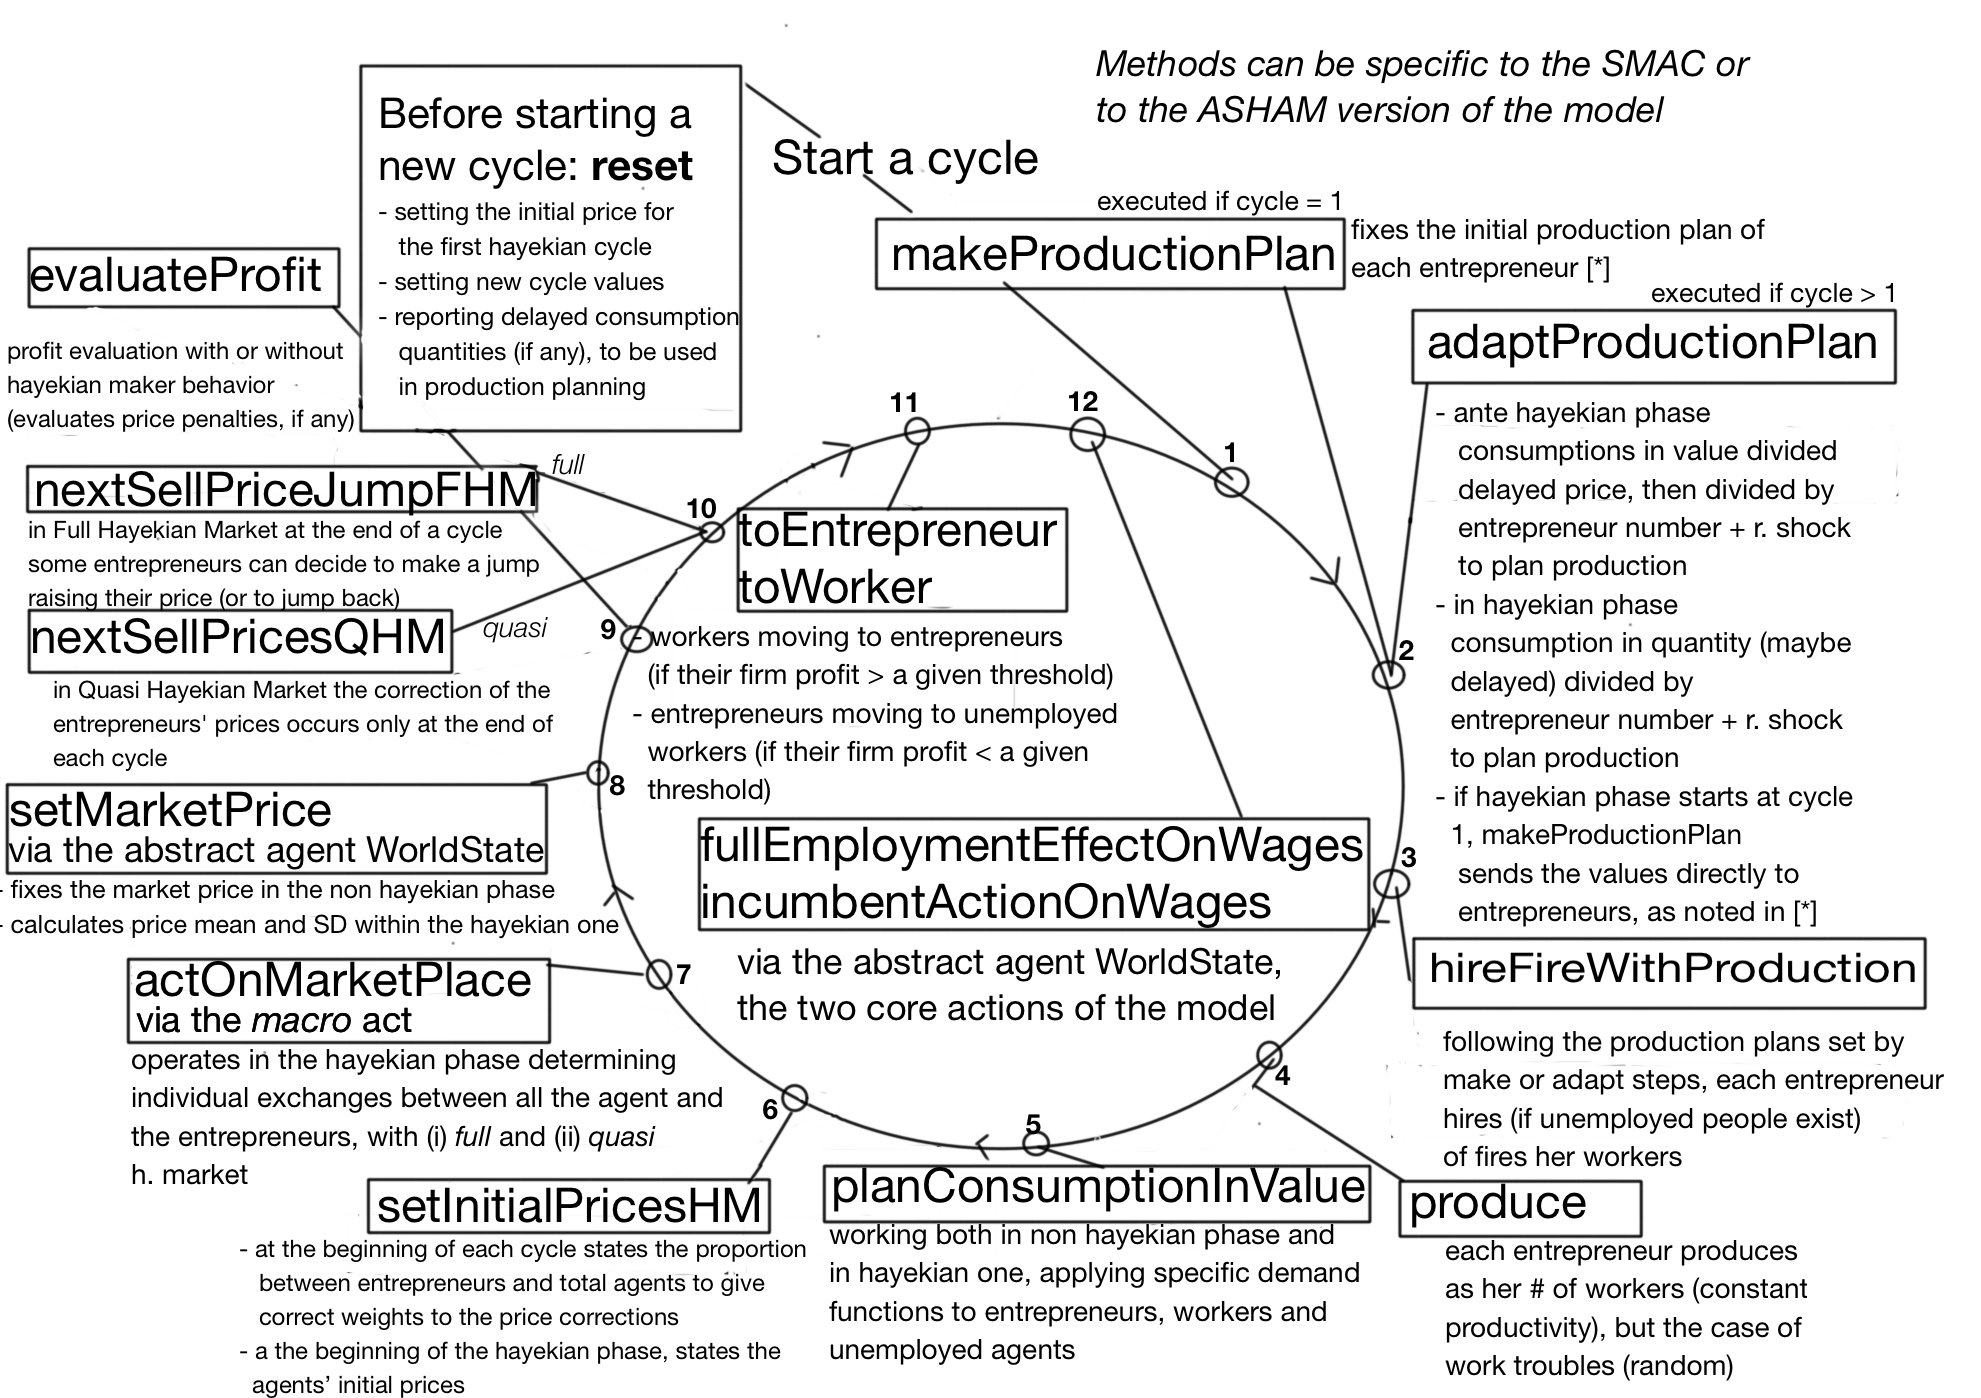
\includegraphics[width=0.85\textwidth]{OligopolyOutline.png}}
\caption{Simulation outline}
\label{outline}
\end{figure}


\end{frame}

\end{document}